\documentclass[11pt,letterpaper]{article}

\usepackage{ctable}

\usepackage{etoolbox}
\makeatletter
\patchcmd{\@verbatim}
  {\verbatim@font}
  {\verbatim@font\small}
  {}{}
\makeatother

\newcommand*\fref[1]{Figure~\ref{fig:#1}}
\newcommand*\tref[1]{Table~\ref{table:#1}}
\newcommand*\sref[1]{Section~\ref{sec:#1}}
\newcommand*\eg{e.g.,~}
% \newcommand*\ie{i.e.,~}
\newcommand*\vs{vs.~}
\newcommand*\viz{viz.~}

% failed attempt to use \citet in SI - used successfully in main paper
% will hard-code the 2 refs where needed
%\usepackage{natbib}
%\newcommand*\citet[1]{{\citeauthor{#1}~\cite{#1}}}

\renewcommand{\thetable}{S\arabic{table}}
\renewcommand{\thesection}{S\arabic{section}}
\newcommand*\ie{i.e.,~}

\setlength{\parindent}{0em}
\setlength{\parskip}{1em}

\title{Scaffold-Based Analytics: Enabling Hit-to-Lead Decisions by
  Visualizing Chemical Series Linked Across Large Datasets}
\author{Deepak Bandyopadhyay$^{\dagger}$, Constantine Kreatsoulas$^{\dagger}$
  Pat G. Brady$^{\dagger}$, \\
  Joseph Boyer$^{\dagger}$, Zangdong He$^{\dagger}$, 
  Genaro Scavello Jr.$^{\dagger}$,\\
  Tyler Peryea$^{\ddagger}$,
  Ajit Jadhav$^{\ddagger}$,
  Dac-Trung Nguyen$^{\ddagger}$,
  Rajarshi Guha$^{\ddagger}$\\
\\
$^{\dagger}$ GlaxoSmithKline, 1250 S. Collegeville Rd, Collegeville,
PA 19426 \\
\\
$^{\ddagger}$ National Center for Advancing Translational Science, \\
9800 Medical Center Drive, Rockville, MD 20850}

\begin{document}

\begin{center}
  {\huge \textbf{Supplementary Information}}
\end{center}
\begin{minipage}{\textwidth}
   \maketitle
\end{minipage}

\newpage 

\section{NCATS R-group tool output files}
\label{sec:ncats-r-group}

\begin{table}[h]
  \centering
  \begin{tabular}[h]{lp{0.75\linewidth}}
    \hline
    \textbf{Column Name} & \textbf{Description} \\
    \hline
    ScaffoldID & Numeric scaffold identifier. Each scaffold occurs only
    once, and data columns are aggregated for all molecules containing the
    scaffold \\
    Structure & Scaffold SMILES without R-groups attached \\
    RgroupLabels & A comma separated list of R-group labels for
    all R-groups associated with the scaffold \\
    ScaffoldScore & A quantitative assessment of the scaffold quality.
    See Section \ref{sec:scaffold-metrics} \\
    Complexity & A number that captures increasing size and complexity of
    scaffolds. See Section \ref{sec:scaffold-metrics}.  \\
    Count & Number of molecules that share this scaffold \\
    \hline
  \end{tabular}
  \caption{A description of the fixed columns of the scaffold file generated
    by the NCATS R-group tool. Additional columns may be present which
    correspond to aggregated property columns. Thus for each
    property of the input molecules, we compute the mean and standard
    deviation of that property for all molecules containing the
    scaffold. These values are reported in columns labeled \texttt{X} and
    \texttt{$X_{sd}$}, where \texttt{X} is the property name.}
  \label{table:scaffoldfilecolumns}
\end{table}

\begin{table}[h]
  \centering
  \begin{tabular}[h]{lp{0.75\linewidth}}
    \hline
    \textbf{Column Name} & \textbf{Description} \\
    \hline
    ScaffoldID & Numeric scaffold identifier (corresponding to
  the {\it ScaffoldID} column in the scaffold file, Table \ref{table:scaffoldfilecolumns}) \\
  MolID & Numeric or text molecule identifier (name). Each molecule is
  repeated once for each scaffold that it occurs in \\
  Structure & Molecule structure in SMILES format \\
  $R_1, \ldots, R_n$ & R-group SMILES, with \*-atoms at attachment
  points. By default we limit to $n = 21$ \\
  \hline
  \end{tabular}
  \caption{A description of the columns in the R-group decomposition
    file generated by the NCATS R-group tool.}
\end{table}


\newpage

\section{Scaffold metrics}
\label{sec:scaffold-metrics}

The NCATS R-group tool is designed to fragment a collection of
molecules. In addition to the fragmentation procedure it computes a
series of scaffold metrics, described in Table
\ref{table:scaffoldfilecolumns}. In this section we provide some
details about the \textit{ScaffoldScore} and \textit{Complexity}
metrics.

The \textit{ScaffoldScore} is an empirical metric designed to
summarize a scaffold (or more generally, a fragment) and the compounds
containing the scaffold. Specifically, we define it as  
\begin{equation}
  \label{eq:1}
  S = -\log_{10} \Bigg( \sqrt{ N_{\mathrm{core}} \times \frac{N_{m}}{N} \times
    \frac{1}{\sqrt{\sigma}} \times \frac{1}{R} }  \, \Bigg)
\end{equation}
where $N_{\mathrm{core}}$ is the atom count of the scaffold,
$N_{m}$ is the size of the member set for the scaffold,
$N$ is the total number of molecules used as input, $R$ is the number
of R-groups identified for this scaffold and $\sigma$ is a measure of
how close the members are to the scaffold and is defined as
\begin{equation}
  \label{eq:2}
  \sigma = \sum_{i=1}^{N_m} ( A_i - N_{\mathrm{core}} )^2
\end{equation}
where $A_i$ is the atom count of the $i$'th molecule in the scaffolds
member set.  In summary, the score for a scaffold is higher if it is
larger, with fewer R-groups and with member molecules that are
relatively close to the scaffold and cover a large fraction of the
input set.

The \textit{Complexity} metric is an implemention of the empirical
complexity metric described by Barone and Channon \cite{Barone2001}.
\textit{Complexity} can be used to prune away scaffolds that are too
simple, by setting a cutoff such as 100.

\newpage 

\section{NCATS R-group tool input preprocessing}
\label{sec:ncats-prepro}
Here are the implementation details specific to summarizing screening datasets such as TCAMS and Kinase X successfully with the NCATS R-group tool:
\begin{itemize}

\item Convert ligand efficiency columns (LE/LLE) to LE\_x10 (multiply by 10). Otherwise it will be rounded to one decimal place while summarizing (eg. $0.3 \pm  0.1$), which isn't useful. The conversion was done using a formula in Excel prior to converting the dataset from CSV to SDF. Summarized LE\_x10 columns may be back-converted to LE by dividing by 10 in a Spotfire calculated column.  

\item Convert integer columns that we are interested in summarizing to floating point format, \ie append a ``.0'' to these integer values. Since Pubchem IDs are integers, there is logic built into the NCATS scaffold summarization code to ignore columns containing integers. However, percentage inhibition, IFI (percent), and many other measurements that are useful to aggregate are expressed as integers.  We got around this by matching a pattern in the SDF file and replacing a PCT\_INHIBITION column followed by an integer with the same number followed by ``.0'' using a Unix sed script. This technique helps work around assumptions made by the NCATS code that integers are compound IDs, and aggregate these columns.
  
\item If the dataset contains Encoded Library Technology features or similar molecules, ensure that pendant  R-atoms  at building block attachment points are deleted rather than turned to Carbon. We implemented this conversion using a MOE SVL script ``db\_deleteatoms.svl'' written by Barbara Sander at Chemical Computing group. The script will loop through a MOE database and delete all atoms named  A  in a database molecule entry, which are the R-atoms. The same thing can be accomplished in the reader's favorite cheminformatics package if they have to deal with molecules with pending R-atoms.  
\end{itemize}

\newpage 

\section{Molecular frameworks input and preprocessing}
\label{sec:gskfw-prepro}
% maybe this moves back?
The input for our implementation of frameworks is a comma separated text file
with molecules encoded in a SMILES field.  The code was modified by
adding scripts to export the fuzzy clusters in a tabular format rather
than prioritize them into mutually exclusive scaffolds as in
\cite{Harper2004DDclus}. This step produces a file similar to
the R-group decomposition format described for the NCATS R-group tool
in \sref{ncats-r-group}, including the following key columns: \emph{framework
  ID, framework SMILES, molecule ID, SMILES} and
\emph{properties/activities}.  There are no R-group columns simply
because this is not a default computation in our frameworks code.

Bemis-Murcko-like and Recap fragments can be built from datasets within the GSK computational chemistry environment as described in \cite{Harper2004DDclus}:
\begin{itemize}
\item Start with a two column space separated SMILES file, \ie chemblntd\_gsk2\_spc.smi which contains molecule parent smiles (no salt forms) and IDs separated by a space. 
\item Run a Python script to generate framework descriptors for each molecule in this dataset; at GSK this script is called build\_dd.py and uses {JChem} library functions, but the reader will find it easy to put together an equivalent script using their preferred cheminformatics toolkit.  The descriptors output by build\_dd.py include Detail Frameworks (chemblntd\_gsk2\_spc\_df.db) and Recap (chemblntd\_gsk2\_spc\_recap.db). These tab-delimited files contain one line per fragment found in any molecule, listing the fragment SMILES and the molecule ID, with all fragments in the first molecule before all in the second, and so on.
\item Convert the two db files into files listing fragments shared by more than one molecule and not unique to a molecule. The resulting file is sorted so that all molecules containing the same fragment are on contiguous lines. Example Unix script for detailed frameworks:
  \begin{verbatim}
    cat chemblntd_gsk2_spc_df.db | sort -V -t \t -k 1
    | awk '{print $2, $1}' | uniq -D -f 1
    > chemblntd_gsk2_spc_frames_shared.txt
  \end{verbatim}
\item As an optional step we did not implement, a scoring function may be computed from the aggregate activity of a fragment and used to triage frameworks as was done for scaffolds from the NCATS R-group tool.   
    
\end{itemize}

%\newpage 
%
%\section{SNG output postprocessing}
%\label{sec:ncats-SNGprep}
%We wrote a Unix sed script to split the comma-separated subscaffold list among multiple lines, with
%the other fields duplicated, since this format is more amenable to Spotfire
%integration as described in the next section.  This script works as follows:
%\begin{verbatim}
%alias gg="sed 's/^\([0-9]*\t[0-9]*\t[^\t]*\)\t\([0-9]*\)\,\(.*\)$/\1\t\2\
%n\1\t\3/g'"
%cat ChemblNTD.network | gg | gg | gg | gg | gg | gg | awk -F, '{print $1}' 
%    > ChemblNTD_scaffold_multiline.txt
%\end{verbatim} 



\newpage 

\section{Implementation Detail of linking Spotfire tables with different scaffold generation methods}
\label{sec:scaf-table-spotfire}

{\bf Complete Linkage Clustering} adds a Cluster Number to the primary data table. To get the Related Molecules, we simply add a duplicate copy of the primary data table and link it to the original via Scaffold ID. In other words, a Table Relation is entered into Spotfire so that $Main.CLink = Main(2).CLink$.  

{\bf GSK Frameworks} are similar to Clusters, except the one-to-many rather than one-to-one mapping of molecules to frameworks. To get the Related Molecules, we add an original and a duplicate copy of this mapping, and set Relations so that:  
\begin{itemize}
\item $Main.Molecule\_ID = Frames(2).Molecule\_ID$
\item $Frames(2).Framework\_ID = Frames.Framework\_ID$
\end{itemize}

{\bf NCATS R-group Tool} adds an additional Annotation layer, \ie the
scaffold-level summaries in addition to the R-group decomposition
table. In order to enable bidirectional navigation from scaffolds to
molecules, we add both these tables and also a duplicate copy of the
R-group decomposition table. Then Relations are set up as follows
within Spotfire:
\begin{itemize}
\item $Main.Molecule\_ID = RGdecomp(2).Molecule\_ID$
\item $RGdecomp(2).Scaffold\_ID = Scaffolds.Scaffold\_ID$
\item $Scaffolds.Scaffold\_ID = RGdecomp.Scaffold\_ID$
\end{itemize}   

%{\bf Scaffold-Network Generator} adds several additional layers of
%complexity to the preceding methods. The Molecule ID in the primary
%dataset is linked only to the Top-Level Scaffold ID in the ID Map
%file; there exists no reverse mapping from subscaffolds with fewer
%rings deep within the network to related Molecule IDs. Thus we create
%one by assuming one wants to explore at most three levels deeper than
%the top level scaffold, but not connect to other molecules that share
%only a single ring (rather than a larger system of two or more rings)
%with the parent molecule. Thus we add six (three in each direction)
%copies of the Scaffold Network table, two of the ID Map table, and two
%of the primary data table, connecting them using the following logic:
%\begin{itemize}
%\item In the three Forward instances of the Network table, the
%  Scaffold to Subscaffold Mapping already exists. Modify it by
%  truncating (assigning a null subscaffold) when the number of rings
%  is 2 or 1.  \subitem Define a new column that maps a null
%  subscaffold to the same scaffold, to be able to follow the link to
%  downstream tables without diving deeper.
%\item In the three Reverse instances of the Network table, the
%  Subscaffold to Superscaffold mapping needs to be defined by
%  inverting the provided mapping. Thus: \subitem We define in each
%  network table a duplicate scaffold ID field, dupID, so that one
%  instance of the ID can be used to map in either direction without
%  introducing a cycle.  \subitem The mapping from scaffolds in one
%  table ($A$) to superscaffolds in one table higher ($B$) is then
%  recast as one from scaffolds in $B$ to subscaffolds in $A$, using a
%  different set of IDs from the upward links.
%\item The Table Relations are then set up as follows to link Molecules
%  to Related Molecules in the scaffold network: \subitem
%  $Main.Molecule\_ID = ID\_Map(2).Molecule\_ID$ \subitem
%  $ID\_Map.Top\_Level\_Scaffold = NetworkDown(3).Scaffold$ \subitem
%  $NetworkDown(3).SubScaffold = NetworkDown(2).Scaffold$ \subitem
%  $NetworkDown(2).SubScaffold = NetworkDown.Scaffold$ \subitem
%  $NetworkDown.Scaffold = NetworkUp.SubScaffold$ \subitem
%  $NetworkUp.Scaffold = NetworkUp(2).SubScaffold$ \subitem
%  $NetworkUp(2).Scaffold = NetworkUp(3).SubScaffold$ \subitem
%  $NetworkUp(3).Scaffold = ID\_Map.Top\_Level\_Scaffold$ \subitem
%  $ID\_Map.Molecule\_ID = Related
%  Molecules(Copy~of~Main).Molecule\_ID$
%\end{itemize}   
%
%% We emphasize that this approach is just one solution to the problem of
%% linking related molecules in Spotfire.  Several other solutions have
%% been explored by our colleagues, which include: duplicating columns
%% rather than tables; joining and merging all data into one giant table
%% rather than maintaining multiple linked tables; linking up molecules
%% directly to lists of other molecules in a preprocess that happens
%% outside Spotfire (\eg in a script that integrates the data); and using
%% various add-ins for Spotfire such as the internally developed GSK SAR
%% Toolkit and commercial tools from Discngine SA.
 
\newpage 

\section{Qualitative Comparison of Scaffold-Generation Methods and Clustering}\label{sec:qualcomp}
{\bf Complete-Linkage Clustering}: As shown in \fref{clusterlanes}, the defining feature of a partitioning clustering is that every molecule maps to one and only one cluster. Thus if a chemotype is broken up among two or more clusters, using the cluster ID to map Related Molecules can retrieve only neighbors from the same cluster, ignoring the other cluster. This is not ideal for purposes of the visualization and navigation method presented here, as arbitrary neighbors would be excluded depending on how the clustering is defined.  Thus we do not advocate the use of clustering, unless it is a fuzzy clustering where all meaningful class memberships a molecule might have are considered. 

\begin{figure}
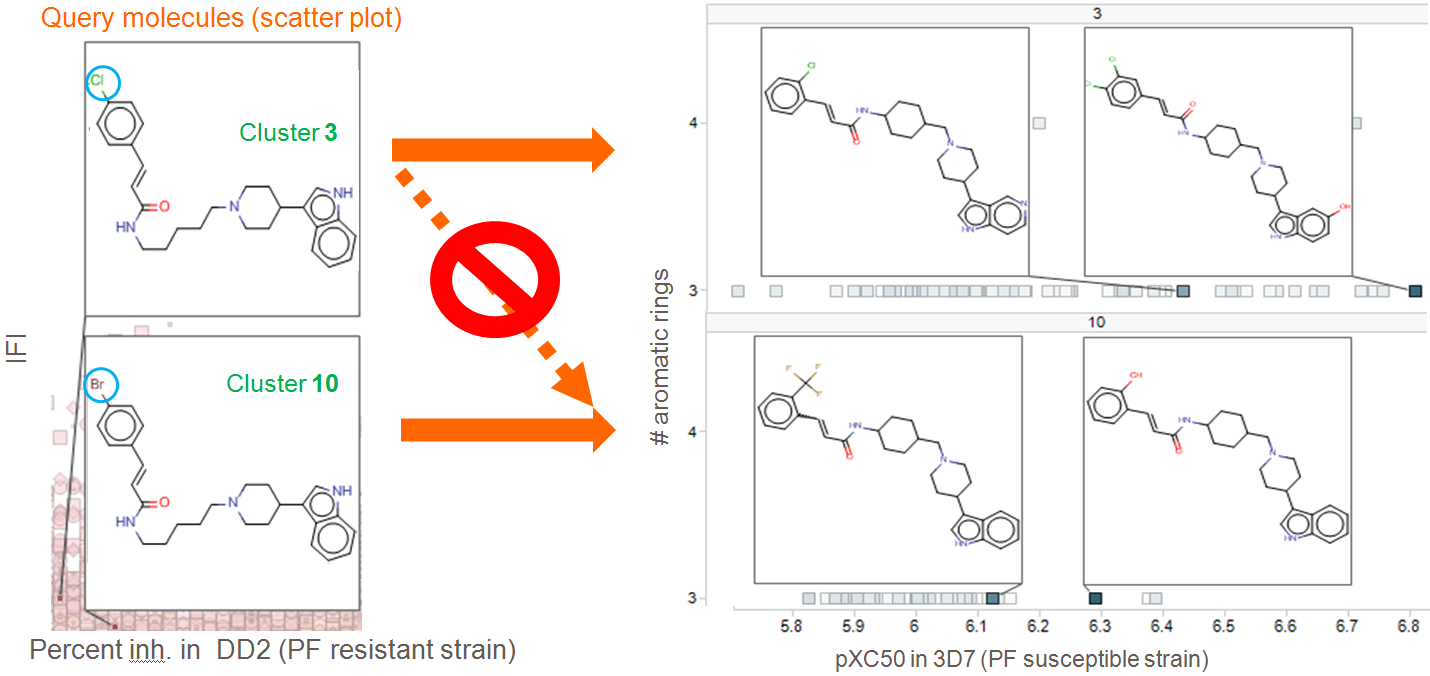
\includegraphics[width=6in]{../fig/clusterlanes.png}
\caption{Illustrating one problem with clustering: bifurcation of related molecules.  When two molecules of the same chemotype differing by a halogen are split across Complete Linkage Clusters, searches of cluster neighbors for one molecule do not find its analogs in the other cluster, \ie the two related clusters are not linked.}
\label{fig:clusterlanes}
\end{figure}



{\bf NCATS R-group tool}: As opposed to the clustering method, 
if any two molecules share a common substructure that meets the standards required of a scaffold by the NCATS method (\eg being bordered by rings on each end), then those molecules will be found to contain that shared substructure as a scaffold and their activities will be used to compute aggregate properties for it. 

{\bf Other Scaffold Generation Methods}: Even though another scaffold generation method (represented here by molecular frameworks as implemented in \cite{Harper2004DDclus}) differed in its implementation details and produced different numbers of scaffolds for the same molecule, it was roughly equivalent in a qualitative sense with regard to the insights obtained during Scaffold Walking. Due to substantial overlap between sets of scaffolds, ring systems responsible for activity of a molecule were generally revealed by either method. However, there were cases where the Frameworks revealed negative information about a fragment being not important for activity that is also useful for a drug discovery scientist. For example, in \fref{frameswalk} a substructure is highlighted that is on the aggregate inactive and could be removed or substituted. This insight is not available from SSSR-based scaffolding methods such as the NCATS R-group tool since they don't define or find that fragment as a scaffold.

\begin{figure}
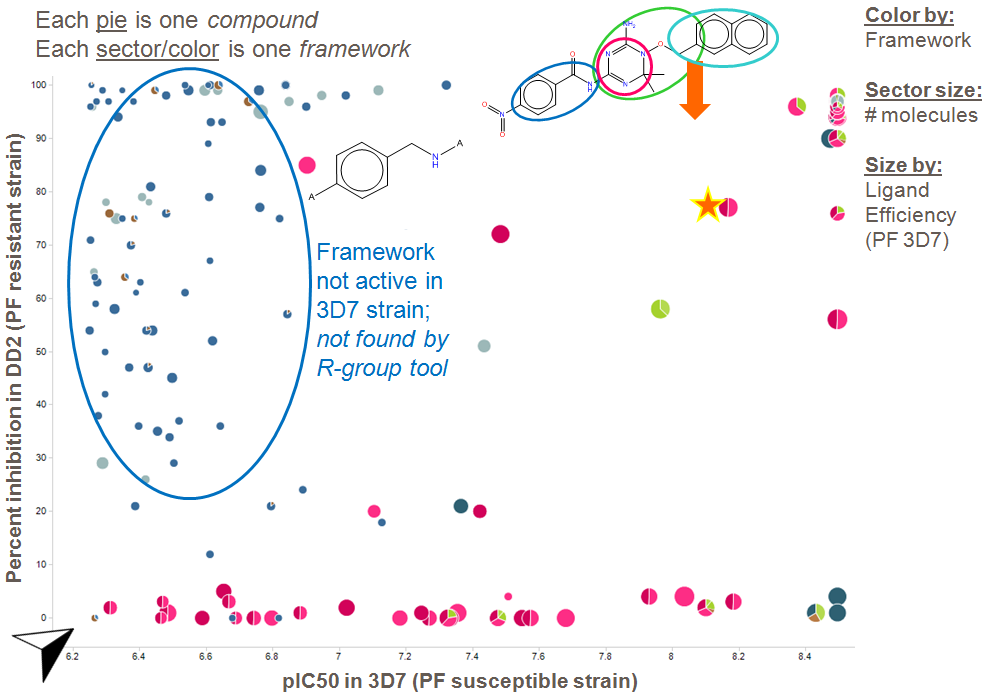
\includegraphics[width=5in]{../fig/mol1_frames_scafpie.png}
\caption{Using Frameworks with the Scaffold Pies visualization. One framework is highlighted that has no equivalent in the NCATS scaffolds, but is shown to reduce activity as related molecules containing it are less active than the parent molecule.   The star symbol shows the location of the parent molecule in this Related Molecules plot, and the compass device at the origin shows the direction of favorable properties (+X and +Y axes).}      
\label{fig:frameswalk}
\end{figure}


To summarize, both multiple-scaffold decomposition methods considered in this study, \ie NCATS R-group Tool and Frameworks give comparable insights when exploring the TCAMS dataset, with some differences stemming from individual substructures that are considered shared scaffolds or not by the individual methods.
%We now explore these overlaps, similarities and differences in the aggregate using the statistical methods described earlier in \sref{statmethod}.

\newpage

\section{Spotfire alternate visualizations and usability tips}
\label{sec:spotviz-trick}
The following additional visualizations have been considered and found useful for NCATS scaffolds and R-groups in analyzing data for GSK projects. They are briefly mentioned below:
\begin{enumerate}
\item {\bf Cross-tables} have been used to list scaffold IDs, compute statistics such as min, max and median activity for each, filter by maximum activity to remove wholly inactive scaffolds, and then prioritize the remaining by drilling down into individual properties
\item {\bf Profile plots} are line graphs used as a visual drill-down mechanism to examine a suite of related assays across all compounds containing a scaffold.They typically have compounds on the X-axis, properties on the Y and are colored by assay name. Figure 6(b) in the main paper shows a profile plot on Kinase X data.
\item {\bf Box plots} are used to visualize the distribution of values of an activity or property for separate scaffolds. Scaffold ID is typically on the X-axis and properties on the Y, allowing multiple scaffolds to be compared side-by-side at a deeper level than just their aggregate activities. 
\end{enumerate}

A few Spotfire techniques were employed to make the users' experience with our Spotfire files more friendly. These have all been tested in TIBCO Spotfire 7.0.2, the version installed at GSK when this work was being concluded.
\begin{itemize}
\item {\bf Structure Visualization:} GSK has a plugin from ChemAxon to visualize structures in tables, labels and tooltips in addition to a dedicated Structure Viewer window. Tooltips were widely employed as they are interactive and allow us to add multiple structure columns, typically a scaffold and the full structure. Labels were used to mark interesting compounds, and structures of cores, R-groups and full molecules depicted in tables helped us create SAR tables directly in Spotfire.
\item {\bf Filtering between related tables:} In addition to creating Table Relations among the Molecules, Scaffolds and Related Molecules tables, we often want to display only scaffolds matching selected molecules of interest, or show only molecules that contain a selected set of scaffolds. This can be achieved by setting the ``Filtering on Related Data Tables'' to either Include Filtered Rows or Exclude Filtered Out Rows.
\item {\bf Tagging:} Used to mark scaffolds selected by the user as being of interest, fulfilling various criteria verified by drilling down into the data behind those molecules.    
\end{itemize}

\newpage 

\section{R code for statistical comparison of scaffold generation methods}
\label{sec:statcode-scafcomp}

The code below expects two files, DDframes.txt (from framework clustering, Method A in the results) and RGD.txt (NCATS R-group tool decomposition, Method B). They both have a column named Compound\_ID. DDframes.txt has a column StrucUniqueID which is computed for example using the DenseRank function in Spotfire, assigning a unique numerical ID to each fragment having different Canonical SMILES.  RGD.txt has a column SCAFFOLD\_ID that is already numerically distinct for each separate scaffold. The code can be generalized for any pair of methods as long as the map from numerical compound IDs to scaffold IDs exists in the input data. 

\begin{verbatim}
#Note: To do the calculations comparing 2 fragmentation methods
#took about 10 minutes of computer time.

#Set working directory to location of the data files
setwd("C:\\Work\\Consulting\\MDR\\Other MDR Issues\\CSC\\FragmentOntologies")
#####################
rm(list = ls()) #Erase anything in R's working memory

DDData <- read.table("DDframes.txt", header = T, sep = "\t")
RGData <- read.table("RGD.txt", header = T, sep = "\t")

#Create a list of compounds shared between two datasets.
#Scores will not make sense if we include non-common compounds

DDCompounds <- unique(DDData$COMPOUND_ID)
RGCompounds <- unique(RGData$COMPOUND_ID)

Compounds <- intersect(DDCompounds, RGCompounds)
# Compounds <- as.numeric(as.character(intersect(DDCompounds, RGCompounds)))
N <- length(Compounds)

#Calculate PI's and common proportions for each compound
  
#Proportions by compound

PropByCompound <- data.frame(CompoundID = rep(NA, N),
			     FragA = rep(NA, N),
			     FragB = rep(NA, N),
                             Ca = rep(NA, N),
                             Cb = rep(NA, N),
                             IntAB = rep(NA, N),
                             UnionAB = rep(NA, N),
                             CommonProp = rep(NA, N),
                             PIa = rep(NA, N),
                             PIb = rep(NA, N),
                             PIaU = rep(NA, N),
                             PIbU = rep(NA, N),
                            FragEffA = rep(NA, N),
                            FragEffB = rep(NA, N))

for (index in 1:N){
  
  PropByCompound$CompoundID[index] <- Compounds[index]
  
  MethodABelongsTo <- DDData[DDData$COMPOUND_ID == Compounds[index],
                            "StrucUniqueID"]
  MethodBBelongsTo <- RGData[RGData$COMPOUND_ID == Compounds[index],
                            "SCAFFOLD_ID"]
							
  PropByCompound$FragA[index] <- length(unique(MethodABelongsTo))
  PropByCompound$FragB[index] <- length(unique(MethodBBelongsTo))
  
  MethodACompoundCluster <- unique(DDData[DDData$StrucUniqueID %in% MethodABelongsTo,
                                   "COMPOUND_ID"])
  MethodBCompoundCluster <- unique(RGData[RGData$SCAFFOLD_ID %in% MethodBBelongsTo,
                                   "COMPOUND_ID"])
  
  PropByCompound$Ca[index] <- length(MethodACompoundCluster)
  PropByCompound$Cb[index] <- length(MethodBCompoundCluster)
  PropByCompound$IntAB[index] <- length(intersect(MethodACompoundCluster,
                                                  MethodBCompoundCluster))
  PropByCompound$UnionAB[index] <- length(union(MethodACompoundCluster,
                                                    MethodBCompoundCluster))
  PropByCompound$CommonProp[index] <- PropByCompound$IntAB[index]/
                                      PropByCompound$UnionAB[index]
  PropByCompound$PIa[index] <- PropByCompound$Ca[index]/PropByCompound$UnionAB[index]
  PropByCompound$PIb[index] <- PropByCompound$Cb[index]/PropByCompound$UnionAB[index]
  PropByCompound$PIaU[index] <- 1 - PropByCompound$Cb[index]/PropByCompound$UnionAB[index]
  PropByCompound$PIbU[index] <- 1 - PropByCompound$Ca[index]/PropByCompound$UnionAB[index]
  PropByCompound$FragEffA[index] <- PropByCompound$Ca[index]/PropByCompound$FragA[index]
  PropByCompound$FragEffB[index] <- PropByCompound$Cb[index]/PropByCompound$FragB[index]
  
}

#Create output -- averages, quantiles, and histograms

ACP <- mean(PropByCompound$CommonProp, na.rm = T)
APIaU <- mean(PropByCompound$PIaU, na.rm = T)
APIbU <- mean(PropByCompound$PIbU, na.rm = T)
AFragEffA <- mean(PropByCompound$FragEffA, na.rm = T)
AFragEffB <- mean(PropByCompound$FragEffB, na.rm = T)

CP95 <- quantile(PropByCompound$CommonProp, c(0.05,0.25,0.5,0.75, 0.95))
PIaU95 <- quantile(PropByCompound$PIaU, na.rm = T, c(0.05,0.25,0.5,0.75, 0.95))
PIbU95 <- quantile(PropByCompound$PIbU, na.rm = T, c(0.05,0.25,0.5,0.75, 0.95))
FragEffA95 <- quantile(PropByCompound$FragEffA, na.rm = T, c(0.05,0.25,0.5,0.75, 0.95))
FragEffB95 <- quantile(PropByCompound$FragEffB, na.rm = T, c(0.05,0.25,0.5,0.75, 0.95))

ACP
APIaU
APIbU
AFragEffA
AFragEffB

CP95
PIaU95
PIbU95
AFragEffA95
AFragEffB95

write.table(PropByCompound,"PropByCompound.txt",sep="\t",row.name=F,col.name=T)
#########################################################################################

################# Plot #####################
attach(PropByCompound)

hist(FragA,main="FragA")
hist(FragB,main="FragB")
hist(CommonProp,main="CommonProp")

plot(CommonProp~UnionAB)
plot(CommonProp~IntAB)
plot(Ca~Cb)

plot(UnionAB, IntAB)
plot(FragA + FragB, CommonProp)

detach(PropByCompound)

\end{verbatim}

\newpage


\bibliographystyle{unsrt}
\bibliography{bibliography}

\end{document}

